\documentclass[11pt,a4paper]{article}
\usepackage[utf8]{inputenc}
\usepackage[T1]{fontenc}
\usepackage{lmodern}
\usepackage[margin=2.3cm]{geometry}
\usepackage{amsmath,amssymb}
\usepackage{graphicx}
\usepackage{booktabs}
\usepackage{float}
\usepackage{xcolor}
\usepackage{tikz}
\usetikzlibrary{arrows.meta,positioning}
\usepackage{caption}
\usepackage{listings}
\graphicspath{{../outputs/figures/}}
\lstset{basicstyle=\ttfamily\small,frame=single,columns=fullflexible}
\setlength{\parskip}{4pt}

\title{\textbf{Swing-up and Fuzzy Balancing of an Inverted Pendulum on a Cart}\\[4pt]
\large Mamdani vs.\ Sugeno controllers and a Simscape Multibody digital twin}
\author{Marco Buonfantino\\ \small Artificial Intelligence Based Control -- BME}
\date{October 2026}

\begin{document}
\maketitle

\begin{abstract}
An inverted pendulum on a cart is brought from the hanging position to the upright position and balanced there. The swing-up uses an energy-based law; near the upright position a supervisor switches to a fuzzy balancing controller made of two PD-like fuzzy controllers (angle loop and cart loop) with 7 linguistic values and 49 rules each. The same rule base is implemented both as a Mamdani system (max--min inference, centroid defuzzification) and as a zero-order Sugeno system, and the two are scaled with a linear-quadratic regulator so that they are equivalent for small errors. The controllers are tested in MATLAB in four scenarios (nominal, external push, model mismatch, sensor noise) and in a Simulink model whose plant is a Simscape Multibody \emph{digital twin} with 3D visualization, validated against the analytical model. Both fuzzy controllers swing up and balance the pendulum in every scenario; the Mamdani controller needs less control effort and is markedly less sensitive to measurement noise.
\end{abstract}

\section{Introduction}
The inverted pendulum on a cart is a classical benchmark for nonlinear control: it is open-loop unstable in the upright position, under-actuated (one force, two degrees of freedom) and strongly nonlinear over the whole range of motion. The task here has two parts:
\begin{enumerate}
  \item \textbf{swing-up}: starting from the hanging position, bring the pendulum close to the upright position using a limited force and a limited track;
  \item \textbf{balancing}: stabilize the pendulum upright and bring the cart back to the centre of the track.
\end{enumerate}
The balancing is done with fuzzy logic controllers (FLCs) designed following the structure seen in the course: normalization, fuzzification, inference with a rule base, defuzzification and denormalization. Two inference systems are compared on the same rules: Mamdani and Sugeno. Finally, the closed loop is reproduced in Simulink with a Simscape Multibody model of the mechanism, which acts as a digital twin with a 3D view.

\section{System model}
\subsection{Equations of motion}
The state is $z = [x,\ \dot x,\ \theta,\ \dot\theta]^T$, where $x$ is the cart position and $\theta$ the pendulum angle ($\theta = 0$ upright, $\theta = \pi$ hanging down, positive when the tip moves towards $+x$). The pendulum is a uniform rod with centre of mass at distance $l$ from the pivot and inertia $I$ about its centre of mass. The Lagrange equations are
\begin{align}
(M + m)\,\ddot x + m l \cos\theta\,\ddot\theta - m l \dot\theta^2\sin\theta + b\dot x &= F,\\
m l\cos\theta\,\ddot x + (I + m l^2)\,\ddot\theta - m g l\sin\theta + c\dot\theta &= 0,
\end{align}
which are solved for $\ddot x$ and $\ddot\theta$ at every time step (\texttt{model/pendulum\_dynamics.m}).

\begin{table}[H]
\centering
\caption{Model and controller parameters (\texttt{model/pendulum\_params.m}).}
\begin{tabular}{llr|llr}
\toprule
Cart mass $M$ & kg & 0.5 & Force limit $F_{\max}$ & N & 15\\
Pendulum mass $m$ & kg & 0.2 & Track half length & m & 1.0\\
Pivot--CoM distance $l$ & m & 0.3 & Sampling time $T_s$ & ms & 10\\
Rod inertia $I = m(2l)^2/12$ & kg\,m$^2$ & 0.006 & Swing-up gain $k_e$ & -- & 10\\
Cart friction $b$ & N\,s/m & 0.1 & Max swing-up acceleration & m/s$^2$ & 4\\
Pivot friction $c$ & N\,m\,s/rad & 0.002 & Catch / release angle & deg & 20 / 46\\
\bottomrule
\end{tabular}
\end{table}

\subsection{Linearization and LQR reference}
Linearizing around the upright equilibrium gives one unstable pole at about $+5.5$~rad/s. A linear-quadratic regulator with $Q = \mathrm{diag}(10, 1, 100, 1)$ and $R = 0.1$ gives
\begin{equation}
F_\mathrm{LQR} = 10\,x + 11.0\,\dot x + 60.0\,\theta + 10.3\,\dot\theta .
\end{equation}
The LQR is \emph{not} used to control the pendulum. It serves only as a reference for scaling the fuzzy controllers (Section~\ref{sec:scaling}). Note the positive sign of the cart gains: to bring the cart back to the centre, the controller first has to tilt the pendulum towards the centre, a typical non-minimum-phase behaviour of this system.

\section{Control architecture}
\begin{figure}[H]
\centering
\resizebox{\textwidth}{!}{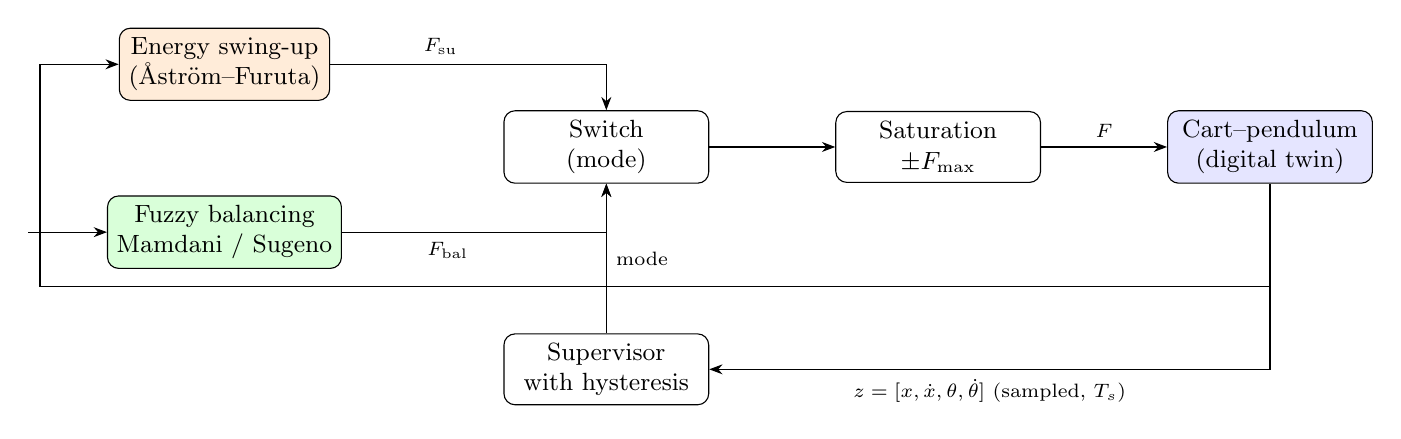
\begin{tikzpicture}[node distance=1.2cm and 1.6cm, >=Stealth,
  box/.style={draw, rounded corners, minimum width=2.6cm, minimum height=0.9cm, align=center, font=\small}]
\node[box, fill=orange!15] (su) {Energy swing-up\\(Åström--Furuta)};
\node[box, fill=green!15, below=of su] (fz) {Fuzzy balancing\\Mamdani / Sugeno};
\node[box, right=2.2cm of su, yshift=-1.05cm] (sw) {Switch\\(mode)};
\node[box, right=of sw] (sat) {Saturation\\$\pm F_{\max}$};
\node[box, fill=blue!10, right=of sat] (pl) {Cart--pendulum\\(digital twin)};
\node[box, below=1.9cm of sw] (sv) {Supervisor\\with hysteresis};
\draw[->] (su) -| node[pos=0.2, above, font=\scriptsize]{$F_\mathrm{su}$} (sw);
\draw[->] (fz) -| node[pos=0.2, below, font=\scriptsize]{$F_\mathrm{bal}$} (sw);
\draw[->] (sw) -- (sat); \draw[->] (sat) -- node[above, font=\scriptsize]{$F$} (pl);
\draw[->] (sv) -- node[right, font=\scriptsize]{mode} (sw);
\draw[->] (pl.south) |- node[pos=0.75, below, font=\scriptsize]{$z = [x,\dot x,\theta,\dot\theta]$ (sampled, $T_s$)} (sv.east);
\draw[->] (pl.south) ++(0,-1.3) -| ([xshift=-1.0cm]su.west) -- (su.west);
\draw[->] ([xshift=-1.0cm]fz.west) -- (fz.west);
\end{tikzpicture}}
\caption{Control architecture. The supervisor selects the swing-up law far from the upright position and the fuzzy controller near it.}
\end{figure}

\section{Energy-based swing-up}
The energy of the pendulum, zero at the upright rest position, is
\begin{equation}
E = \tfrac12 (I + m l^2)\,\dot\theta^2 + m g l\,(\cos\theta - 1),
\end{equation}
so $E = -2mgl$ when the pendulum hangs at rest. Its time derivative is $\dot E = -m l\,\ddot x\,\dot\theta\cos\theta - c\dot\theta^2$, hence choosing the cart acceleration
\begin{equation}
a = \mathrm{sat}_{a_{\max}}\!\big(k_e\,(E - E_\mathrm{ref})\,\dot\theta\cos\theta\big) - k_x x - k_v \dot x
\end{equation}
makes the energy grow monotonically towards $E_\mathrm{ref}$ (the last two terms keep the cart near the centre of the track). The acceleration is converted into a force by inverse dynamics. A small margin $E_\mathrm{ref} = 0.1\,mgl$ above the upright energy is used: with $E_\mathrm{ref} = 0$ the pumping vanishes as the energy approaches the target, and with a heavier pendulum and more friction (Scenario~3) the pendulum stopped just short of the catch region. With the chosen gains the pendulum reaches the upright region after three swings in about 4.3~s, with the cart within $\pm 0.3$~m.

\section{Fuzzy balancing controller}
\subsection{Structure}
Controlling four state variables with a single FLC would need $7^4 = 2401$ rules. As suggested in the course for PID-like controllers, the problem is split into two PD-like FLCs whose outputs are summed:
\begin{equation}
F_\mathrm{bal} = K_{u,\theta}\;\mathrm{FLC}_\theta\!\Big(\frac{\theta}{\theta_{\max}}, \frac{\dot\theta}{\dot\theta_{\max}}\Big) + K_{u,x}\;\mathrm{FLC}_x\!\Big(\frac{x}{x_{\max}}, \frac{\dot x}{\dot x_{\max}}\Big).
\end{equation}
Inputs are normalized to $[-1, 1]$ (and saturated), the normalized output $u\in[-1,1]$ is denormalized by the output gain $K_u$.

\subsection{Fuzzification and rule base}
Each normalized input has 7 linguistic values NB, NM, NS, Z, PS, PM, PB: triangles centred at $k/3$, $k = -3,\dots,3$, with trapezoidal shoulders at the ends (Fig.~\ref{fig:mf}). The rule base is the classical PD-like table $u = \mathrm{sat}(e + \Delta e)$ (Table~\ref{tab:rules}): 49 rules of the form
\emph{if $e$ is $E_i$ and $\Delta e$ is $\Delta E_j$ then $u$ is $U_{\mathrm{sat}(i+j)}$}.

\begin{figure}[H]
\centering
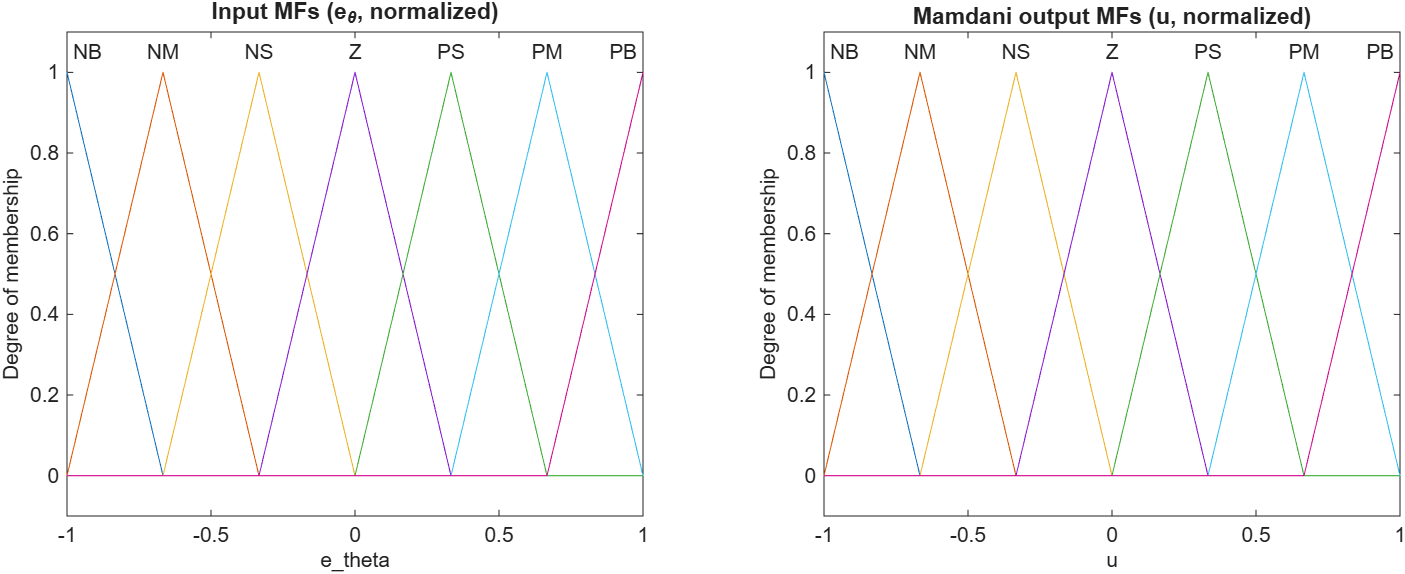
\includegraphics[width=\textwidth]{membership_functions.png}
\caption{Membership functions of the normalized inputs (left) and of the Mamdani output (right).}
\label{fig:mf}
\end{figure}

\begin{table}[H]
\centering
\caption{Rule base (same for both loops and both inference methods): output label as a function of $e$ (rows) and $\Delta e$ (columns).}
\label{tab:rules}
\begin{tabular}{c|ccccccc}
$e \backslash \Delta e$ & NB & NM & NS & Z & PS & PM & PB\\\hline
NB & NB & NB & NB & NB & NM & NS & Z\\
NM & NB & NB & NB & NM & NS & Z & PS\\
NS & NB & NB & NM & NS & Z & PS & PM\\
Z  & NB & NM & NS & Z & PS & PM & PB\\
PS & NM & NS & Z & PS & PM & PB & PB\\
PM & NS & Z & PS & PM & PB & PB & PB\\
PB & Z & PS & PM & PB & PB & PB & PB\\
\end{tabular}
\end{table}

\subsection{Mamdani and Sugeno inference}
For a crisp input $(e^*, \Delta e^*)$ the firing strength of rule $i$ is $\alpha_i = \min(\mu_{E_i}(e^*), \mu_{\Delta E_i}(\Delta e^*))$.
\begin{itemize}
  \item \textbf{Mamdani} (max--min): each rule clips its output set, $\mu_{U_i'}(u) = \min(\alpha_i, \mu_{U_i}(u))$, the clipped sets are aggregated with max and the crisp output is the centre of gravity
  \[ u^* = \frac{\int u\,\mu_U(u)\,du}{\int \mu_U(u)\,du}. \]
  \item \textbf{Sugeno} (zero order): each rule has a constant consequent $c_i$ equal to the centre of the corresponding Mamdani output set, and
  $u^* = \sum_i \alpha_i c_i \,/\, \sum_i \alpha_i$.
\end{itemize}
Using the same antecedents, rules and output centres isolates the effect of the inference and defuzzification method. Fig.~\ref{fig:surf} shows the resulting control surfaces: the Sugeno surface is almost a plane (piecewise multilinear interpolation of the rule consequents), the Mamdani surface is smoother near the corners but shows a characteristic ripple due to the centroid of overlapping clipped sets.

\begin{figure}[H]
\centering
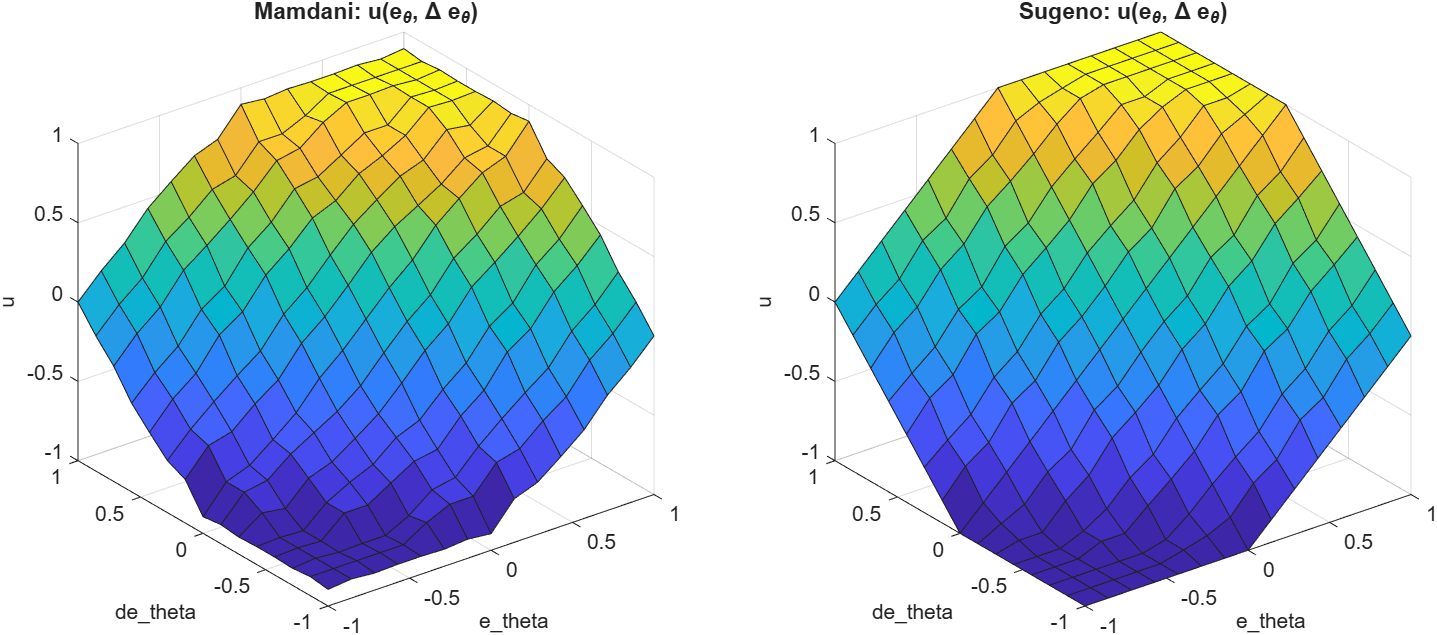
\includegraphics[width=\textwidth]{control_surfaces.png}
\caption{Control surfaces of the angle controller: Mamdani (left) and Sugeno (right).}
\label{fig:surf}
\end{figure}

\subsection{Scaling from the LQR}\label{sec:scaling}
The normalization and output gains determine how aggressive an FLC is. They are chosen so that, for small errors, each FLC has the same gains as the LQR. The slopes of the normalized FLCs at the origin are measured numerically: $s = \partial u/\partial e_n = \partial u/\partial \Delta e_n = 1.39$ for Mamdani and $1.00$ for Sugeno. With $\theta_{\max} = 0.35$~rad (the catch angle) and $x_{\max} = 1$~m (the track half length), matching $K_u s/\theta_{\max} = 60.0$, $K_u s/\dot\theta_{\max} = 10.3$, $K_u s/x_{\max} = 10$, $K_u s/\dot x_{\max} = 11.0$ gives the gains of Table~\ref{tab:gains}. Far from the origin the FLCs saturate smoothly instead of growing linearly like the LQR.

\begin{table}[H]
\centering
\caption{Scaling gains of the fuzzy controllers.}
\label{tab:gains}
\begin{tabular}{lcccccc}
\toprule
 & $\theta_{\max}$ [rad] & $\dot\theta_{\max}$ [rad/s] & $K_{u,\theta}$ [N] & $x_{\max}$ [m] & $\dot x_{\max}$ [m/s] & $K_{u,x}$ [N]\\
\midrule
Mamdani & 0.35 & 2.03 & 15.1 & 1.0 & 0.91 & 7.2\\
Sugeno  & 0.35 & 2.03 & 21.0 & 1.0 & 0.91 & 10.0\\
\bottomrule
\end{tabular}
\end{table}

\section{Switching logic}
The supervisor uses the wrapped angle $\theta_w = \mathrm{atan2}(\sin\theta,\cos\theta)$ and a hysteresis: it switches from swing-up to balance when $|\theta_w| < 0.35$~rad ($20^\circ$) and back to swing-up only if $|\theta_w| > 0.80$~rad ($46^\circ$). The hysteresis prevents chattering between the two controllers when the pendulum is caught near the boundary of the region. The controller runs at $T_s = 10$~ms with zero-order hold.

\section{Digital twin in Simulink}
The Simulink model (\texttt{cartpole\_fuzzy\_twin.slx} in the folder \texttt{simulink}) is generated by the script \texttt{build\_twin\_model.m}. Its plant is a Simscape Multibody model of the mechanism: a rail, the cart on a prismatic joint with viscous friction, the rod on a revolute joint with damping, gravity, force actuation and position/velocity sensing. When the simulation starts, Mechanics Explorer shows the mechanism in 3D. In parallel, the analytical model of Section~2 is driven with the same force: during the swing-up the angles of the two models coincide to within $10^{-4}$~rad, which validates the twin (masses, inertia, axes and sign conventions).

The controller subsystem contains the zero-order hold, a MATLAB Function block with the swing-up law and the supervisor, and two fuzzy subsystems (Mamdani and Sugeno), each with two \emph{Fuzzy Logic Controller} blocks; a constant \texttt{CTRL\_TYPE} selects which one drives the plant (Fig.~\ref{fig:sl}). A 2D dashboard (Fig.~\ref{fig:frames}) animates the logged simulation with live plots and can be exported as a video.

\begin{figure}[H]
\centering
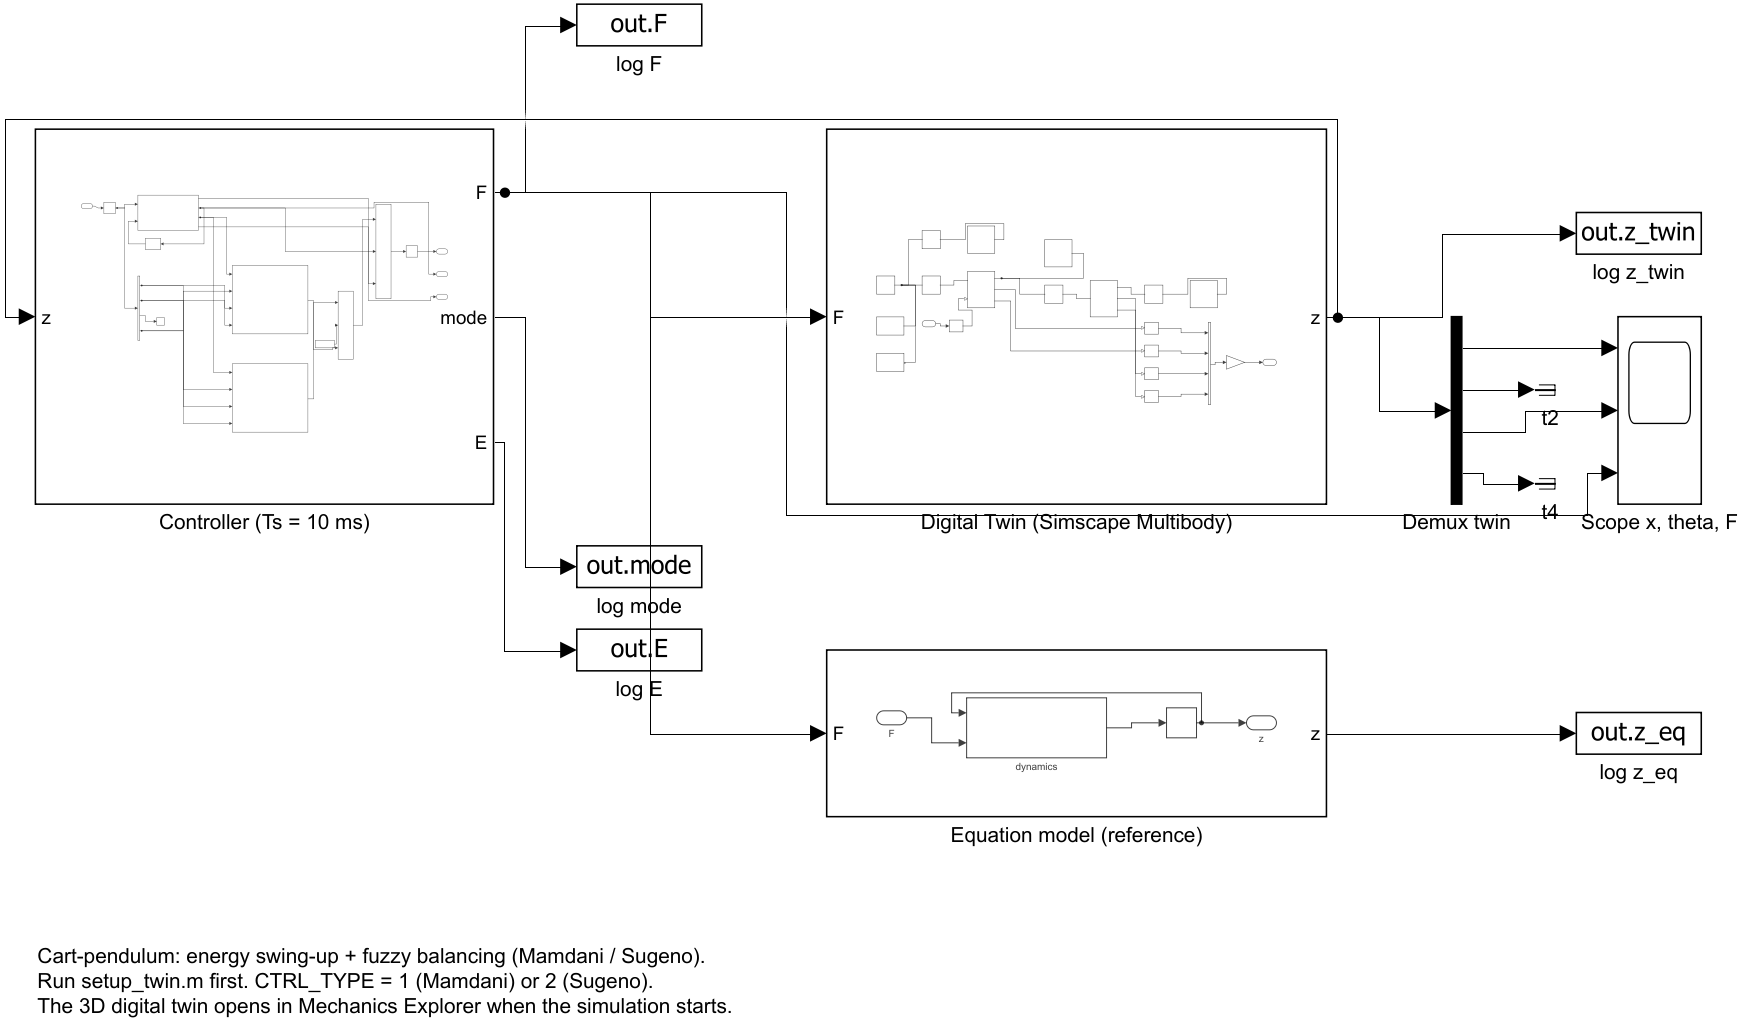
\includegraphics[width=0.95\textwidth]{simulink_top_level.png}\\[4pt]
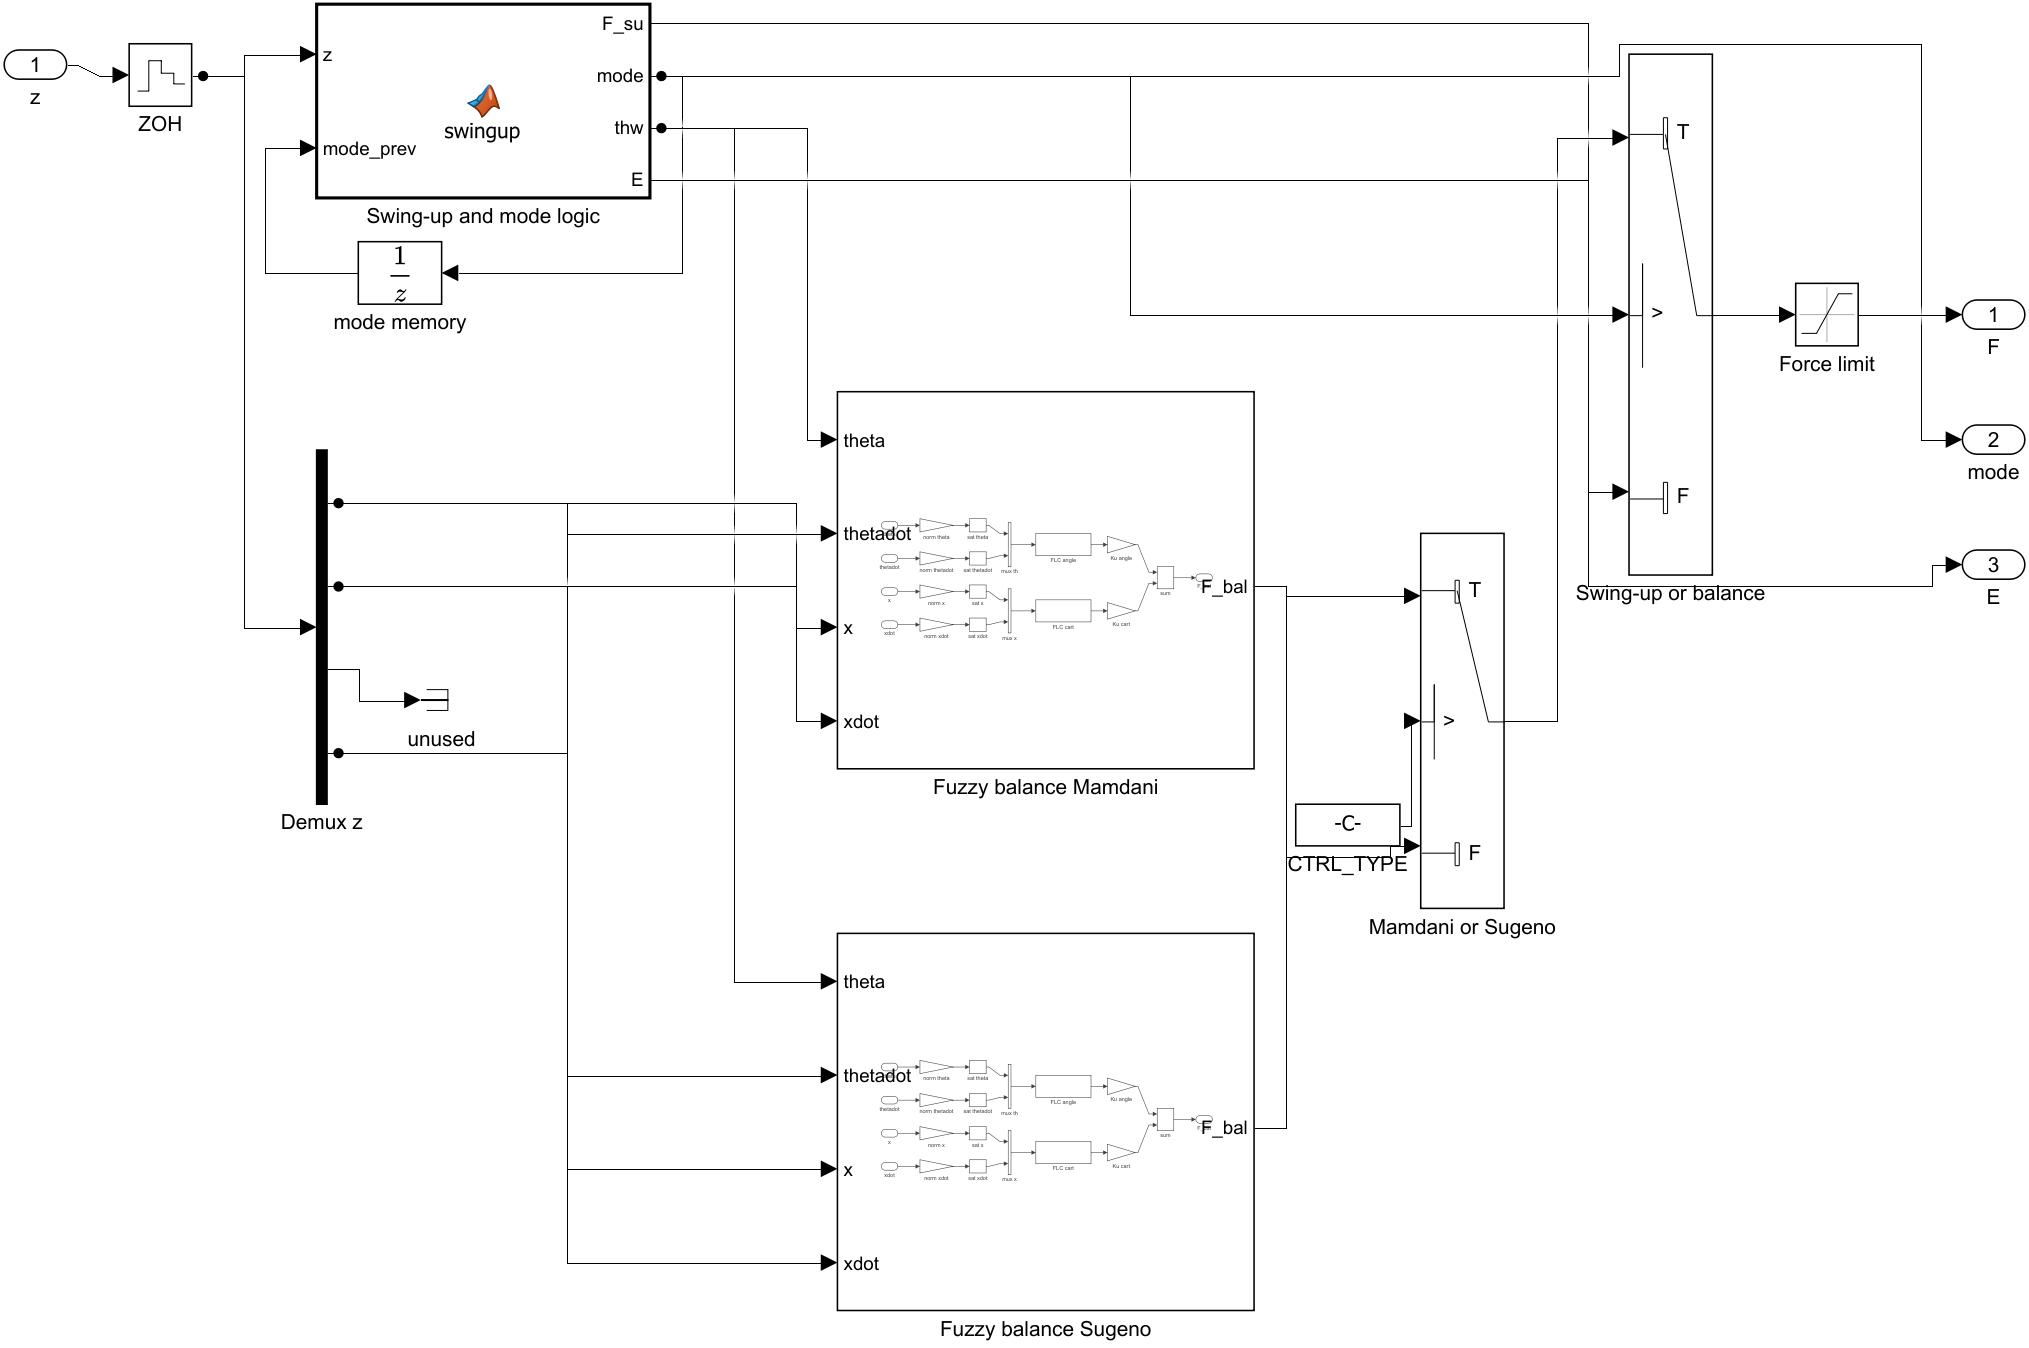
\includegraphics[width=0.95\textwidth]{simulink_controller.png}
\caption{Simulink model: top level (above) and controller subsystem (below).}
\label{fig:sl}
\end{figure}

\begin{figure}[H]
\centering
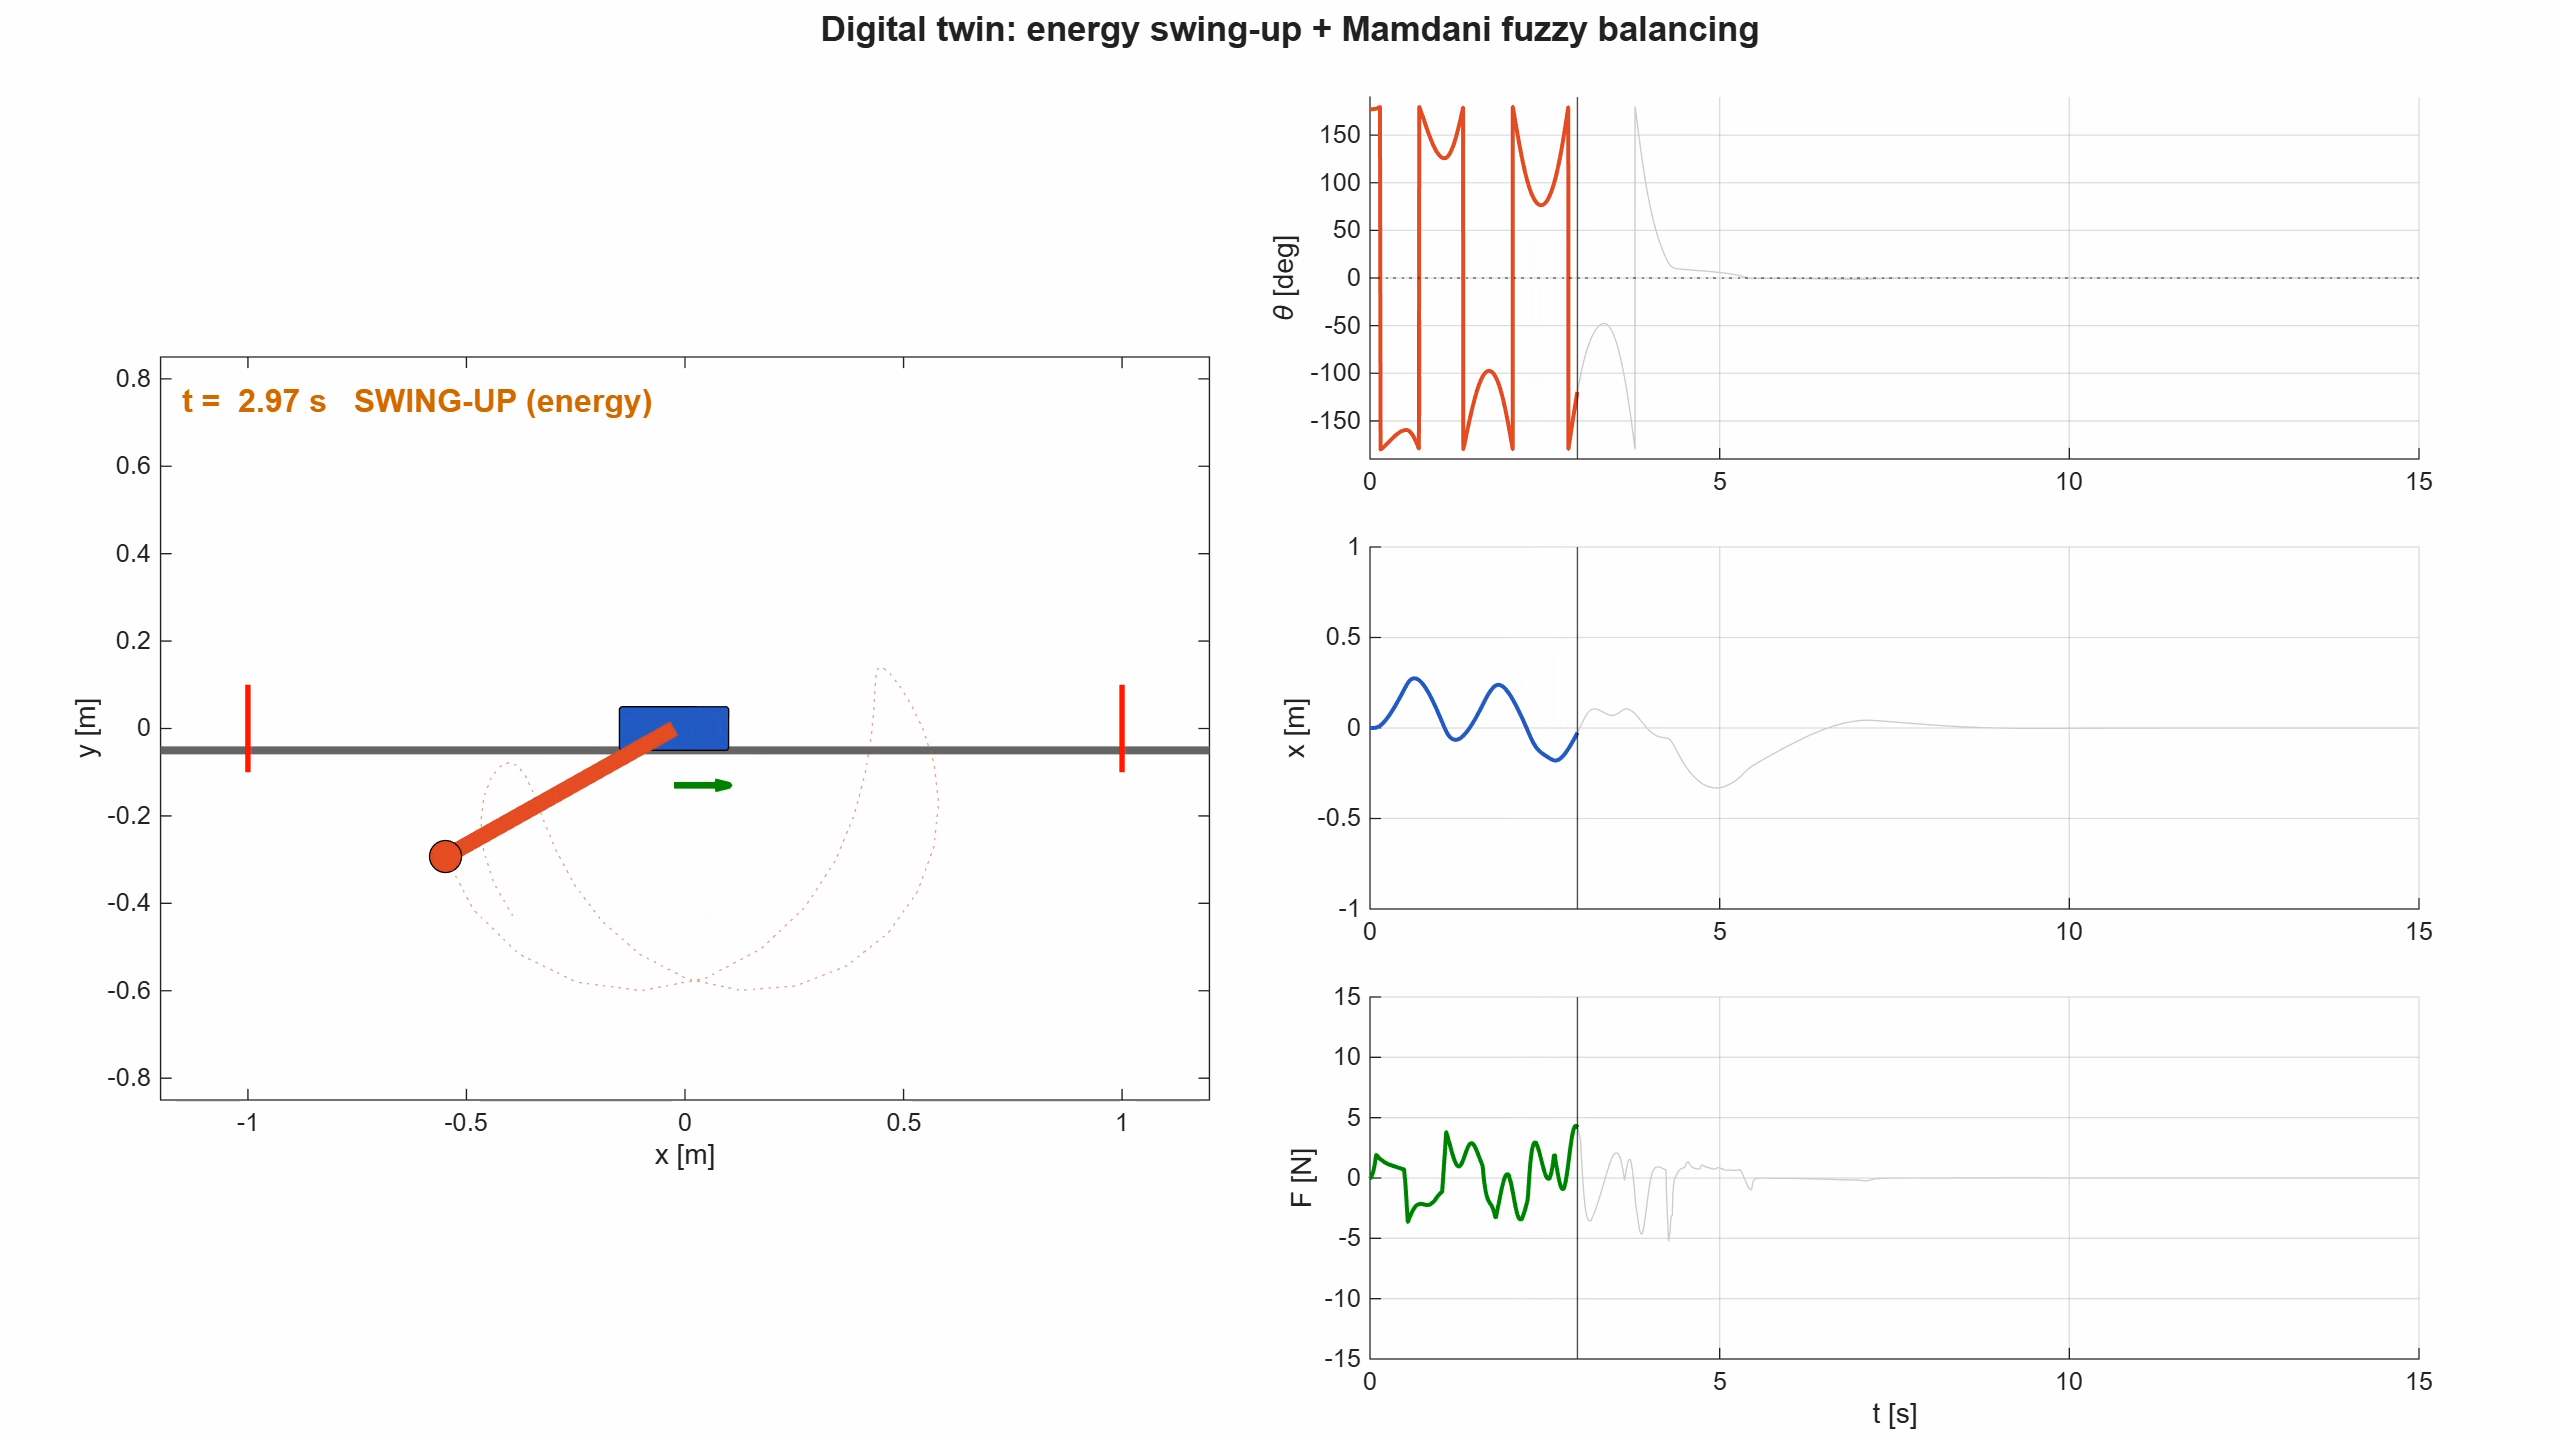
\includegraphics[width=0.49\textwidth]{twin_frame_swingup.png}\hfill
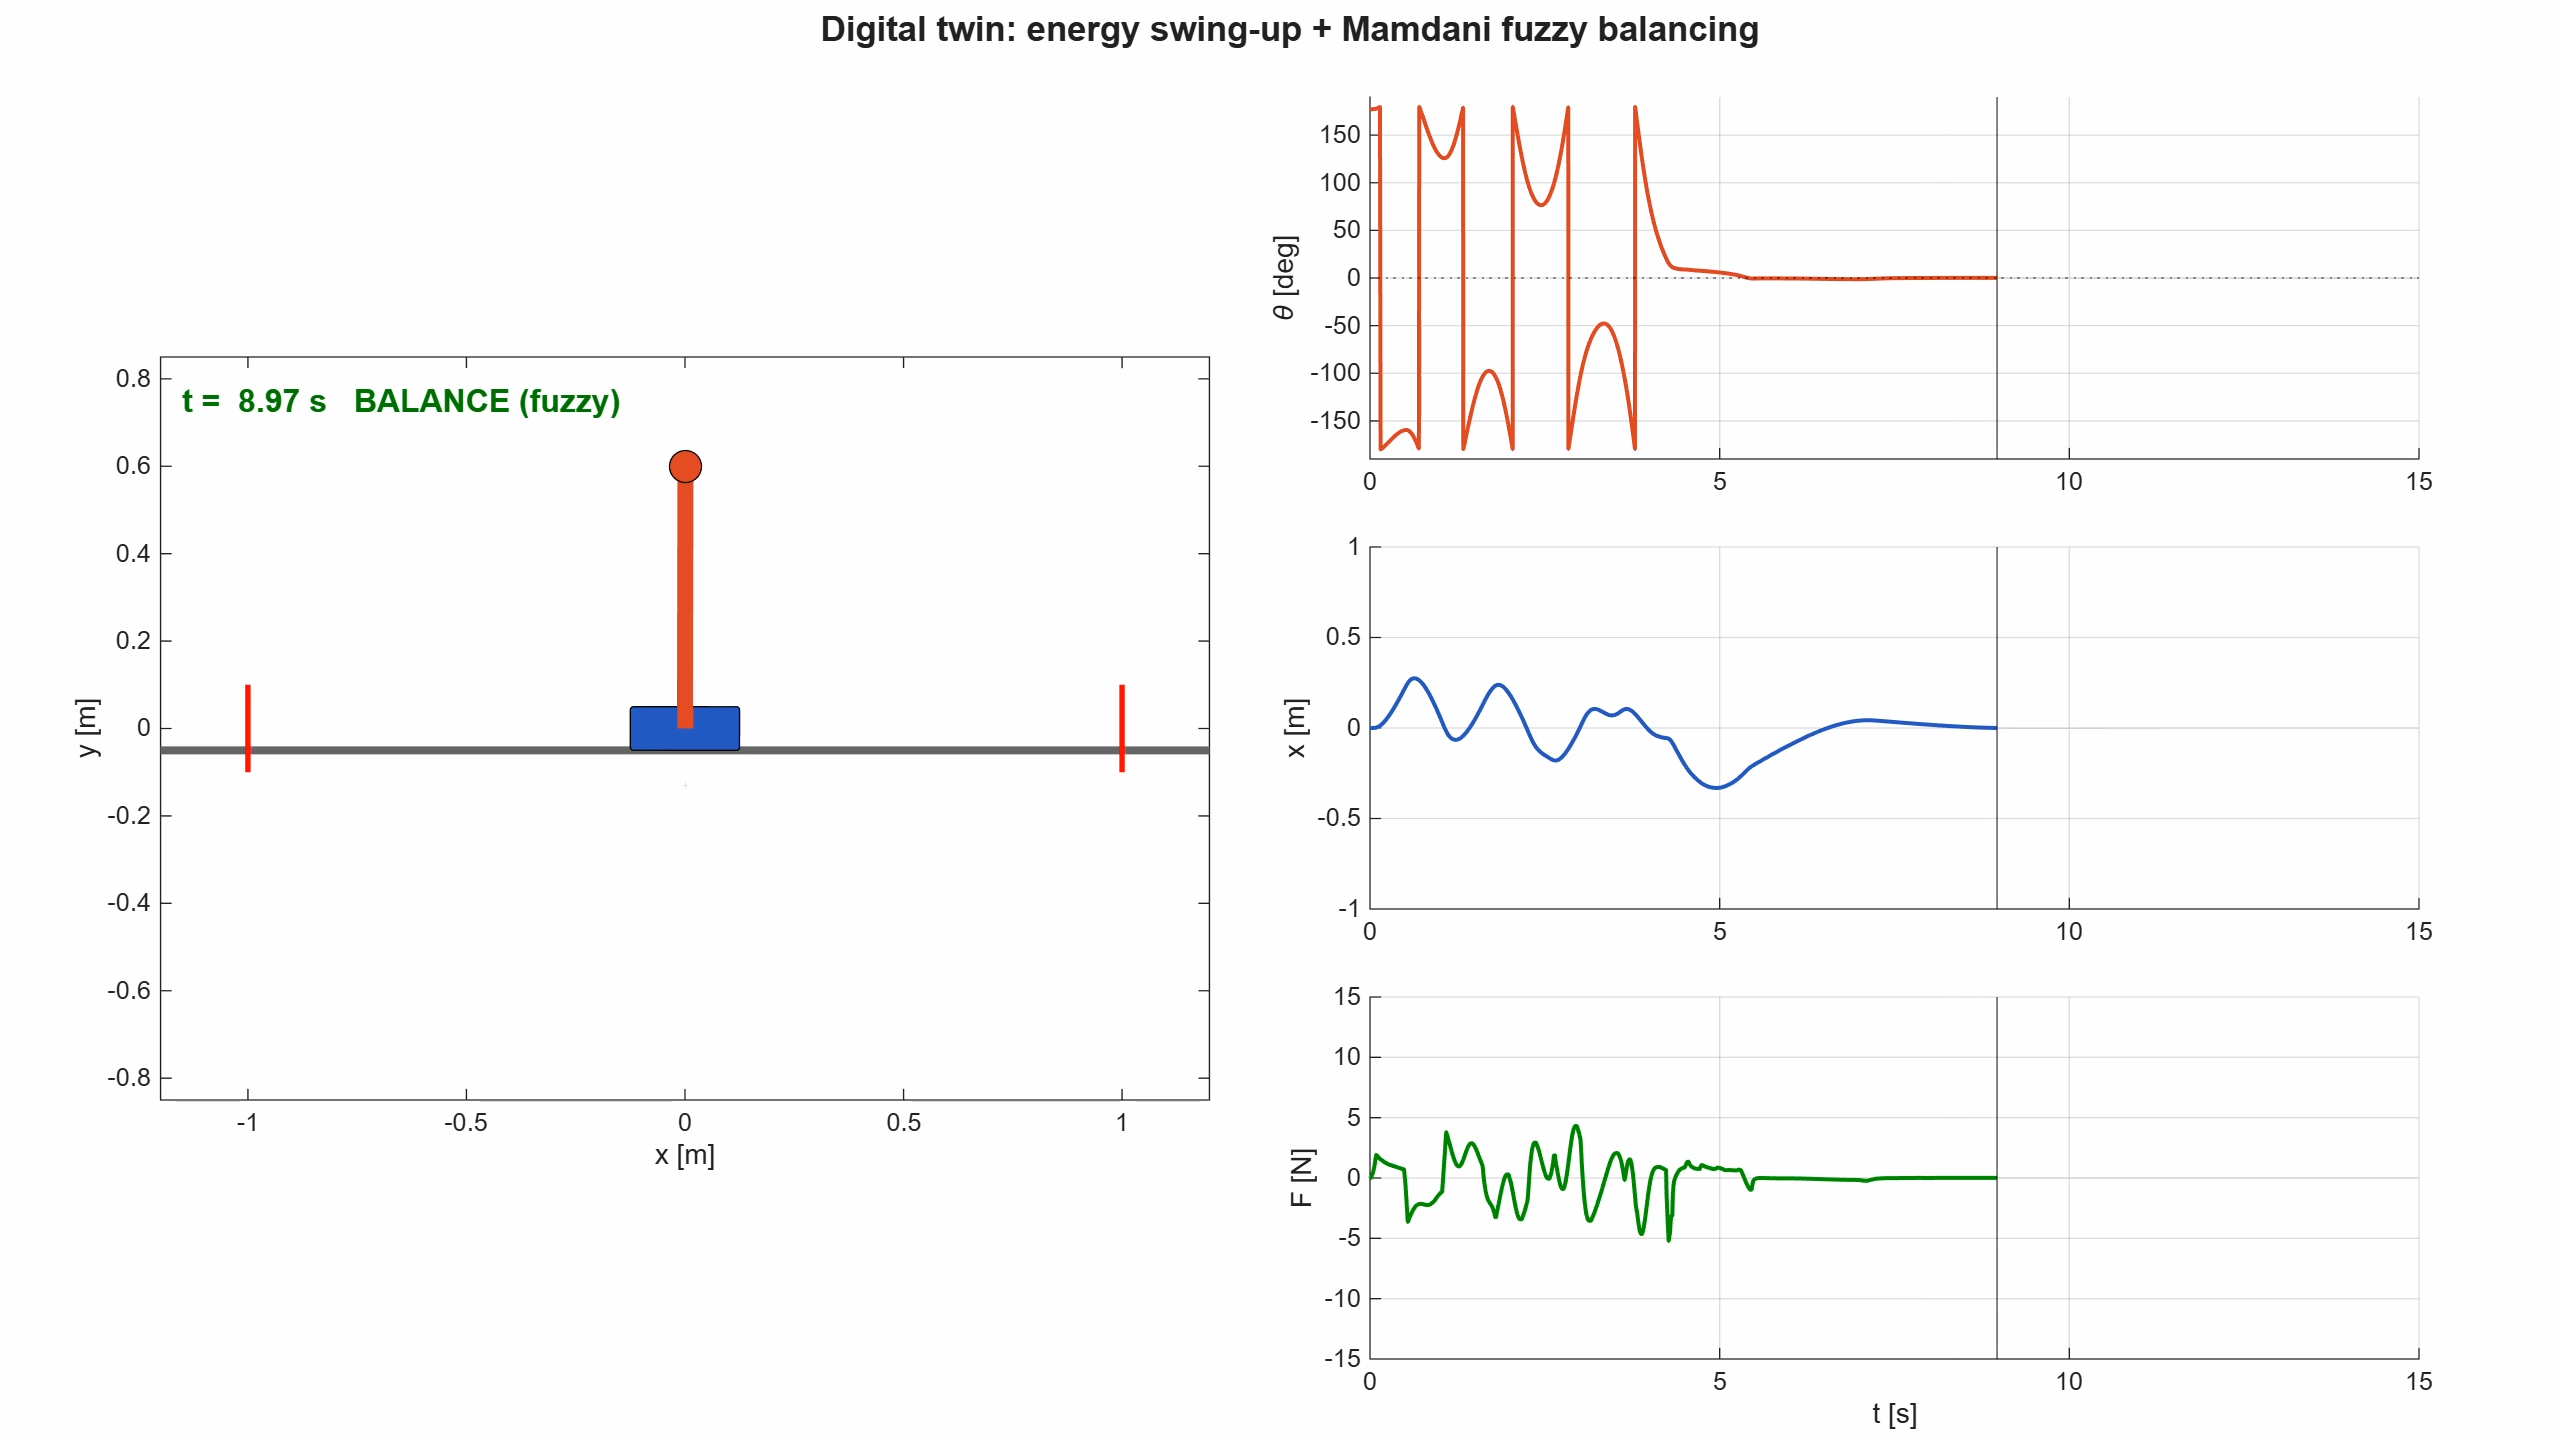
\includegraphics[width=0.49\textwidth]{twin_frame_balance.png}
\caption{2D dashboard of the digital twin (Mamdani): swing-up at $t = 3$~s (left) and balance at $t = 9$~s (right).}
\label{fig:frames}
\end{figure}

\section{Results}
\subsection{Test scenarios}
Both controllers are tested in four scenarios (\texttt{main\_compare.m}), always starting from the hanging position:
\begin{enumerate}
  \item \textbf{Nominal}: the plant equals the model.
  \item \textbf{Push}: at $t = 10$~s the pendulum receives an angular velocity kick of 2.5~rad/s.
  \item \textbf{Model mismatch}: the real pendulum is 50\% heavier and the cart friction is doubled, while the controllers use the nominal parameters.
  \item \textbf{Sensor noise}: Gaussian noise on $x$ (1~mm) and $\theta$ (0.002~rad); velocities are computed by finite differences, as on real hardware.
\end{enumerate}
Table~\ref{tab:res} summarizes the metrics measured after the catch: maximum and RMS angle, RMS cart position, settling time ($|\theta| < 1^\circ$, counted from the catch; in the push scenario it therefore includes the recovery after the push at $t = 10$~s, about 3.2~s), control effort $\int F^2\,dt$ and maximum force.

\begin{table}[H]
\centering
\caption{Results of the four scenarios (generated by \texttt{main\_compare.m}).}
\label{tab:res}
\resizebox{\textwidth}{!}{% generated by visualization/export_latex_table.m -- do not edit by hand
\begin{tabular}{llcccccccc}
\toprule
Scenario & Controller & $t_\mathrm{catch}$ [s] & Balanced & $\max|\theta|$ [$^\circ$] & RMS $\theta$ [$^\circ$] & RMS $x$ [cm] & $t_s$ [s] & $\int F^2$ [N$^2$s] & $\max|F|$ [N]\\
\midrule
nominal & Mamdani & 4.25 & yes & 18.6 & 2.52 & 9.8 & 2.86 & 2.1 & 5.2\\
 & Sugeno & 4.25 & yes & 18.6 & 2.60 & 8.5 & 2.76 & 3.0 & 7.3\\
\midrule
push at t=10 s & Mamdani & 4.25 & yes & 18.6 & 2.99 & 17.9 & 8.91 & 12.4 & 13.7\\
 & Sugeno & 4.25 & yes & 18.6 & 2.99 & 16.9 & 8.88 & 15.2 & 15.0\\
\midrule
model mismatch & Mamdani & 5.79 & yes & 19.1 & 1.78 & 1.0 & 0.29 & 0.4 & 6.0\\
 & Sugeno & 5.79 & yes & 19.1 & 1.75 & 1.0 & 0.29 & 0.7 & 6.0\\
\midrule
sensor noise & Mamdani & 4.26 & yes & 18.8 & 2.28 & 6.8 & 0.95 & 75.9 & 9.1\\
 & Sugeno & 4.26 & yes & 18.8 & 2.32 & 6.5 & 0.93 & 159.3 & 14.3\\
\bottomrule
\end{tabular}
}
\end{table}

\begin{figure}[H]
\centering
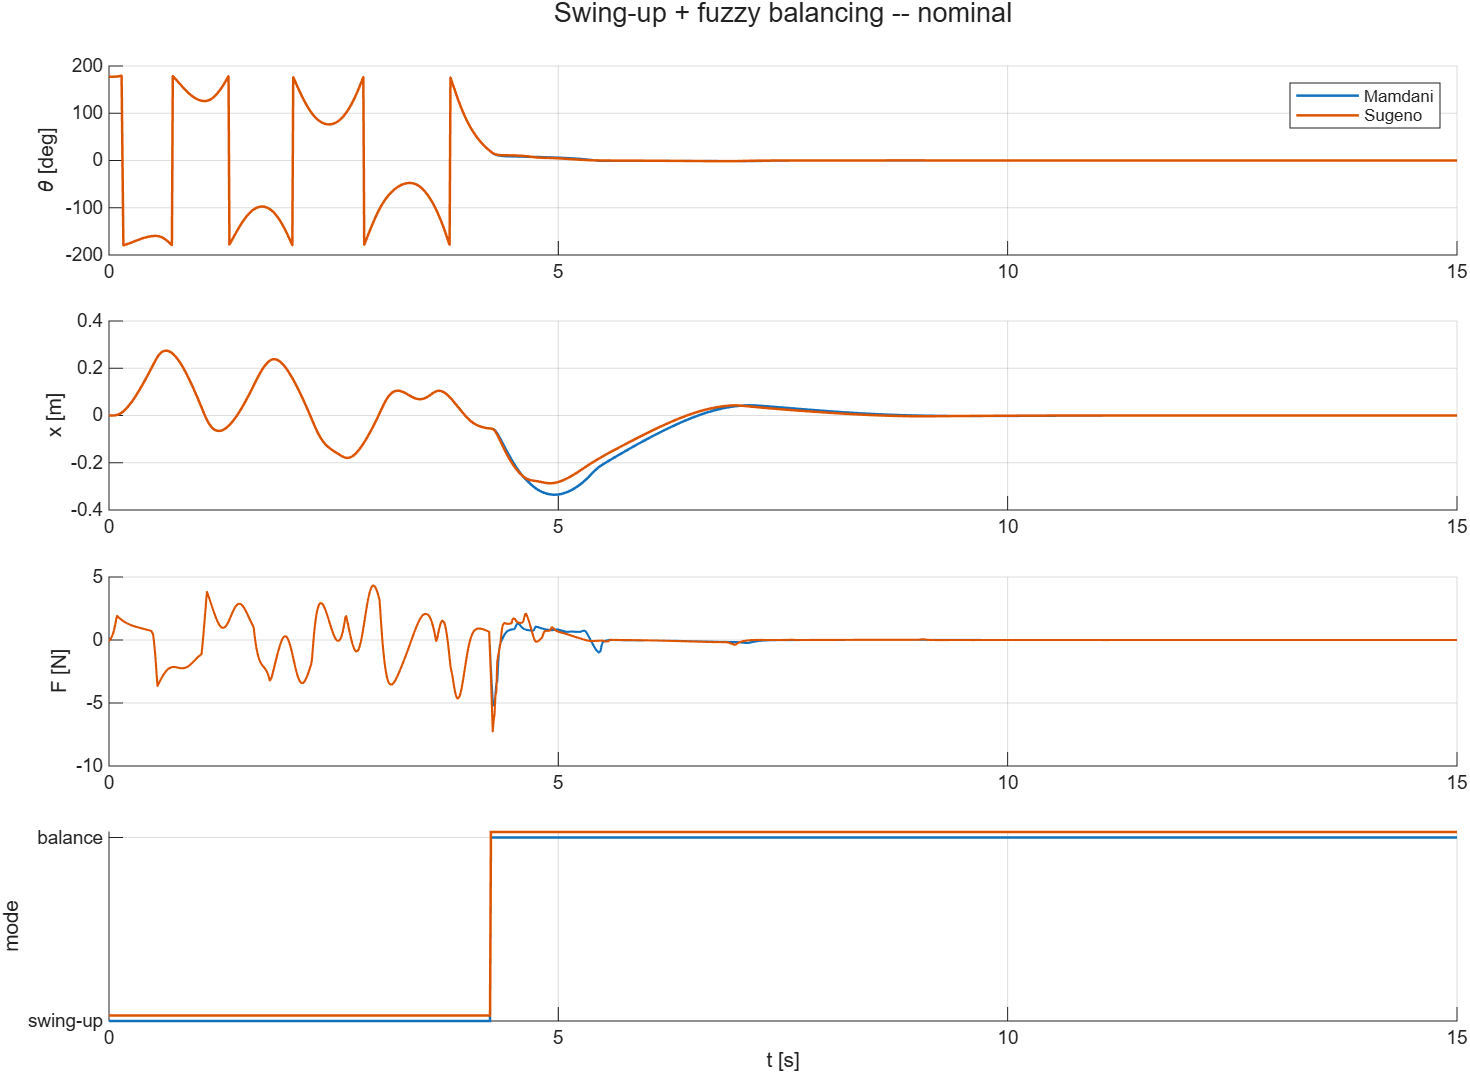
\includegraphics[width=0.49\textwidth]{scenario_1.png}\hfill
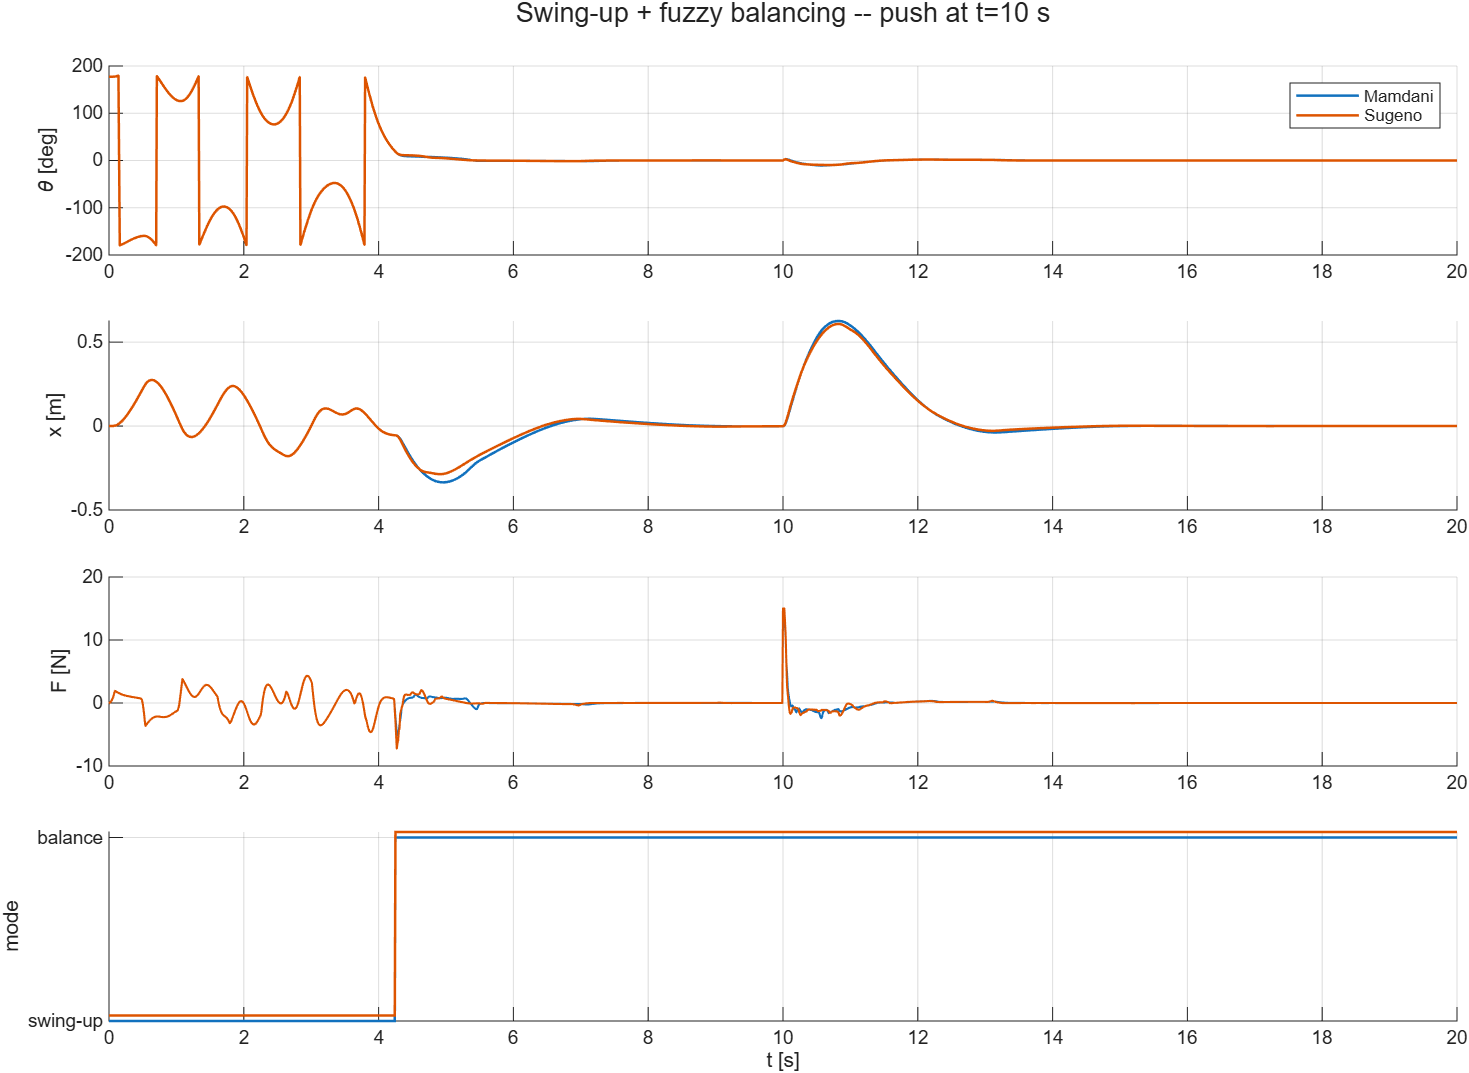
\includegraphics[width=0.49\textwidth]{scenario_2.png}\\[4pt]
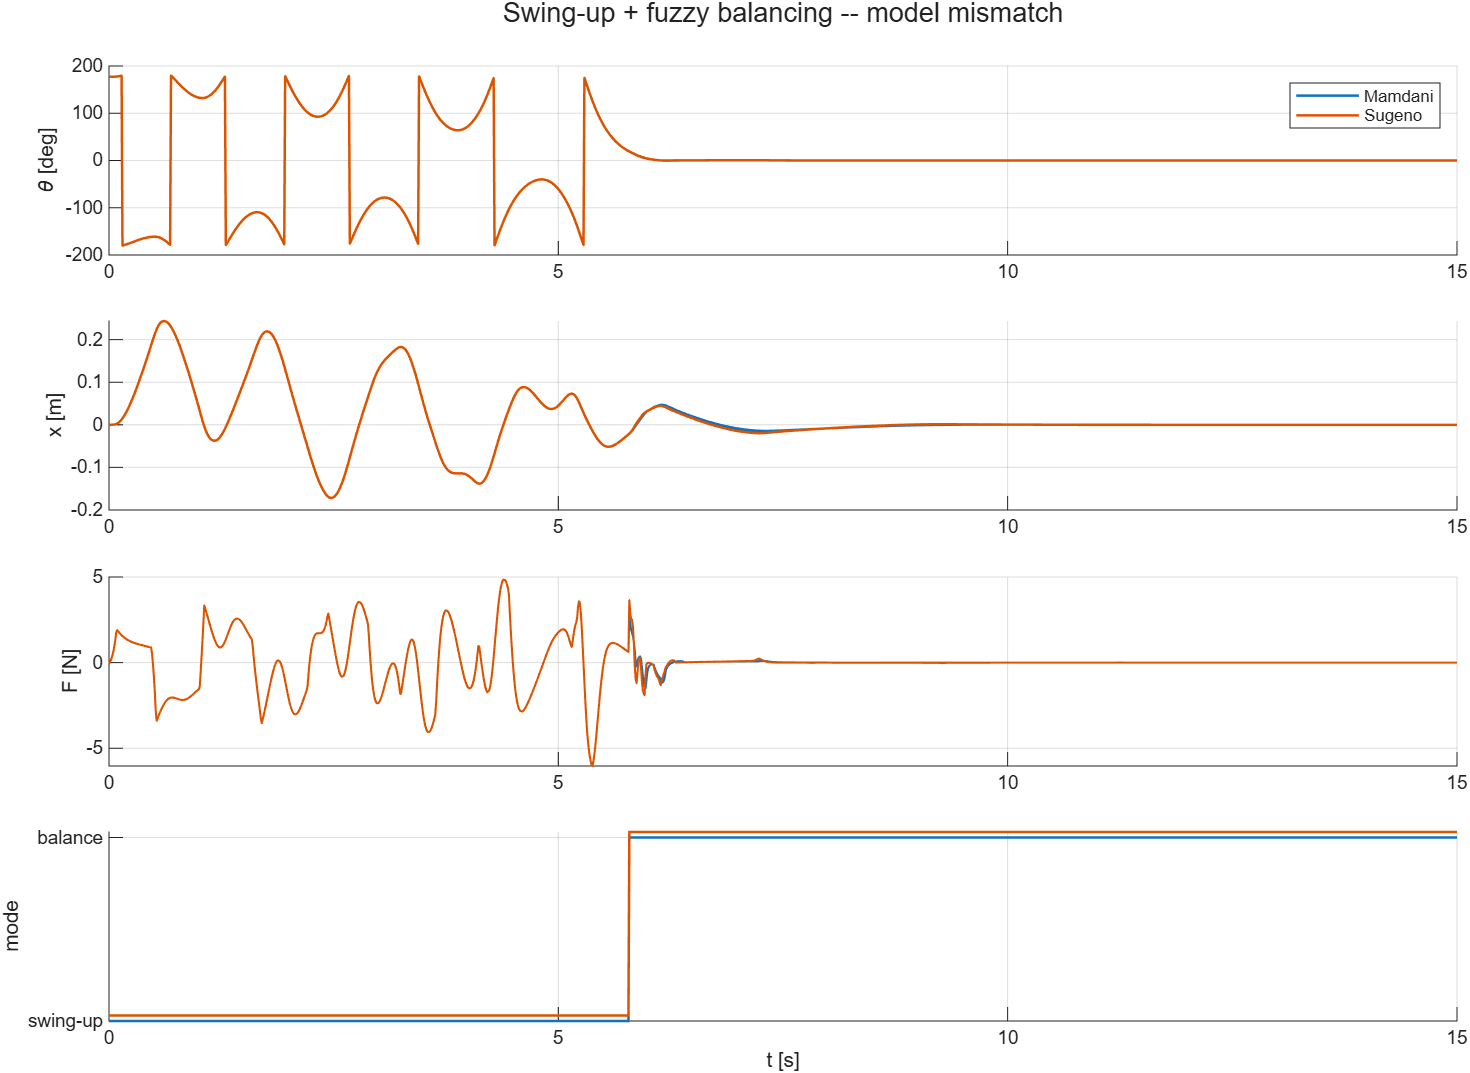
\includegraphics[width=0.49\textwidth]{scenario_3.png}\hfill
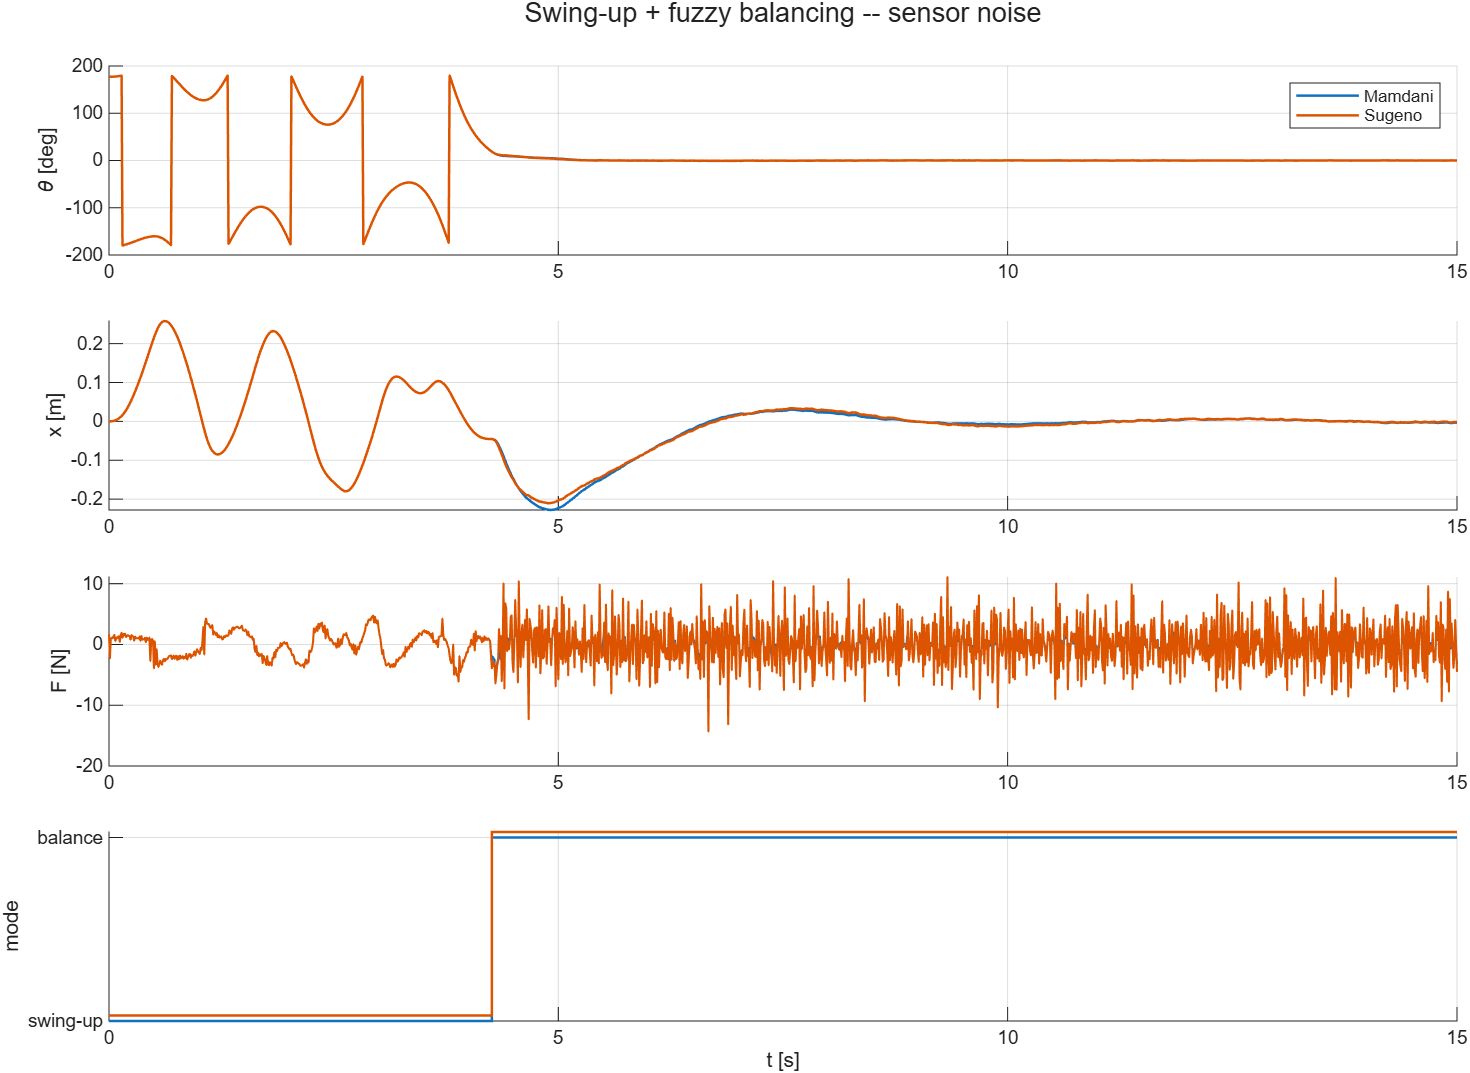
\includegraphics[width=0.49\textwidth]{scenario_4.png}
\caption{Angle, cart position, force and mode in the four scenarios (blue: Mamdani, orange: Sugeno).}
\end{figure}

\subsection{Discussion}
\textbf{Swing-up.} The swing-up does not depend on the fuzzy controller and catches the pendulum after three swings in about 4.3~s (5.8~s with the heavier pendulum). The energy margin makes it robust to the model mismatch; the price is a pendulum that arrives slightly faster at the catch angle and a larger cart excursion right after the catch.

\textbf{Balancing.} Both fuzzy controllers catch and stabilize the pendulum in all four scenarios with a single switch from swing-up to balance, and recover from the external push with the cart staying inside the track. Since they are scaled to the same small-signal gains, their trajectories are very close: the angle errors after the catch differ by less than $0.1^\circ$ RMS.

\textbf{Mamdani vs.\ Sugeno.} The difference is in the control effort. The Mamdani controller needs 18--36\% less effort ($\int F^2 dt$) in the nominal, push and mismatch scenarios, and 52\% less with noisy measurements, where the Sugeno controller also reaches a much higher peak force (14.3~N against 9.1~N); after the push, the Sugeno controller hits the force limit. A likely explanation is visible in the control surfaces: the Mamdani surface is steeper at the origin but flattens away from it (the centroid of overlapping clipped sets moves less than the weighted average of the consequents), so after the LQR scaling its output gain is smaller and large or noisy inputs, such as the finite-difference velocities, produce smaller force variations. The Sugeno controller is computationally cheaper and its surface is easier to interpret as a smooth interpolation of the rule consequents.

\section{Conclusions}
An energy-based swing-up combined with a fuzzy balancing controller swings up and stabilizes the cart--pendulum from the hanging position in about 4~s, and remains stable under an external push, a 50\% heavier pendulum with doubled friction, and noisy measurements. Splitting the balancing into two PD-like FLCs keeps the rule base small (2 $\times$ 49 rules), and scaling them from an LQR gives a systematic tuning method with a clear small-signal interpretation. With identical rules, the Mamdani controller produced smoother control actions and was less sensitive to noise than the Sugeno one. The Simscape Multibody digital twin reproduces the analytical model and makes the behaviour visible in 3D.

Possible extensions: a fuzzy swing-up controller, tuning of the membership functions (e.g.\ with genetic algorithms or ANFIS, also covered in the course), and a real-time test on hardware.

\appendix
\section{How to reproduce}
From the project root in MATLAB (R2026a; Fuzzy Logic Toolbox, Control System Toolbox, Simulink, Simscape, Simscape Multibody):
\begin{lstlisting}
main_compare            % 4 scenarios, Mamdani vs Sugeno -> outputs/
main_twin(1)            % Simulink digital twin with Mamdani (3D + 2D animation)
main_twin(2, true)      % Sugeno, also record outputs/videos/twin_sugeno.mp4
export_latex_table      % refresh the results table of this report
\end{lstlisting}

\end{document}
